\section{Tehnologije}
Za implementaciju rada izabran je Python programski jezik, koji je u posljednih godina dosegnuo visoku popularnost i koristi se u gotovo svim vrstama aplikacija. Interpretirani je jezik visoke razine opće namjene te ima filozofiju dizajna koji naglašava čitljivost k\^oda. Podržava više paradigme programiranja, uključujući objektno orijentirane, imperativne, funkcionalne i proceduralne. Programski jezik se dinamičko kuca (eng. \textit{dynamically typed}), što znači da varijablama se ne određuje tip, ali ako se želi postoji mogućnost izričito ga naglasiti. Posjeduje sveobuhvatnu biblioteku, koja između ostaloga pokriva i područje umjetne inteligencije. Korištenjem se dosta olakšavaju obrade i pripreme podataka za inteligentne agente, te izradu istih. Također, kako se nebi sukobili pakete iz ovog projekta sa paketima iz drugog ili iz sustava, stvorilo se posebno virtualno okruženje samo za ovaj projekt. Pythonov modul koji to omogućuje zove se \emph{virtualenv}.

\subsection{Integrirano razvojno okruženje}
K\^od je pisan u razvojnom okruženju PyCharm koji je jedan od mnogih okruženja Češke tvrtke JetBrains. Glavne značajke su analiza k\^oda, grafički program za otklanjanje pogrešaka, integrirani tester jedininca te integracija s kontrolnim sustavom za verzioniranje. Izgled PyCharm integriranog razvojnog okruženja prikazan je na slici~\ref{fig:pycharm}.
\\[\intextsep]
\begin{minipage}{\linewidth}
	\centering%
	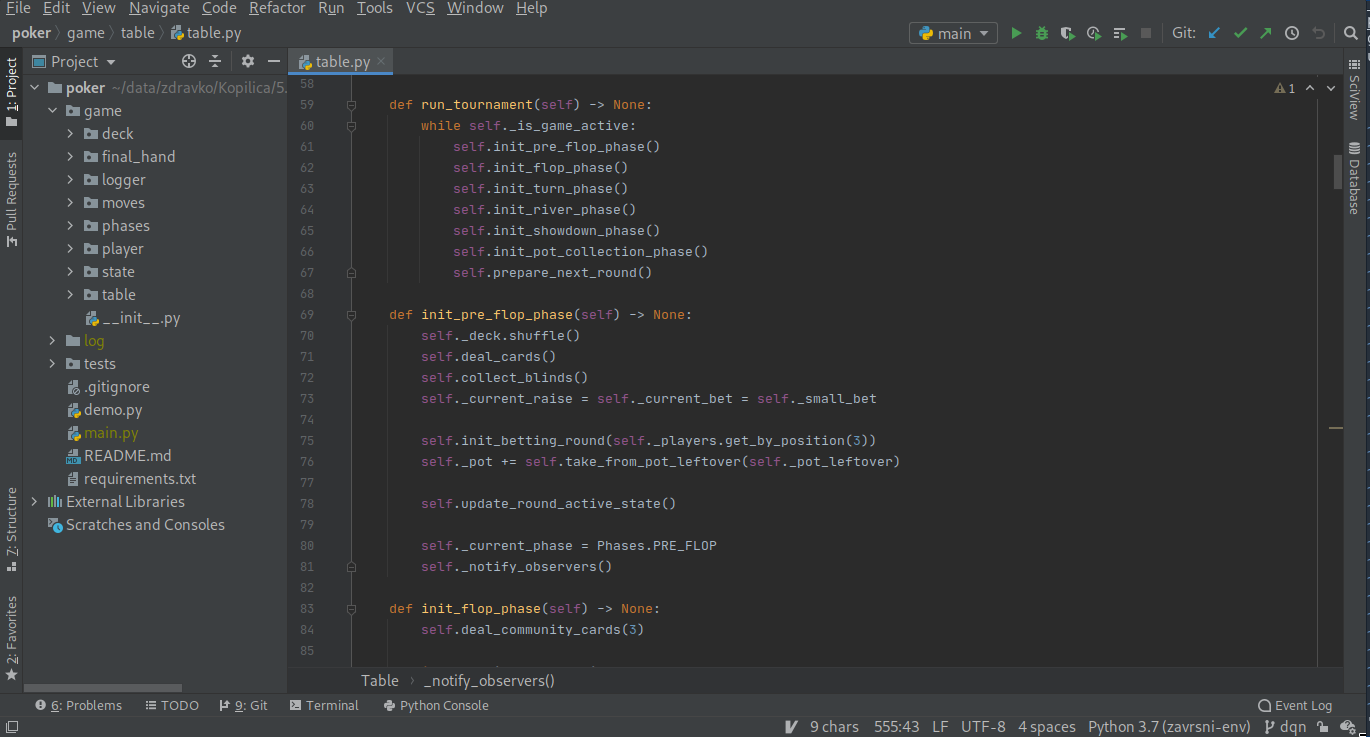
\includegraphics[width=0.8\linewidth,clip=]{images/pycharm.png}%
	\figcaption{Integrirano razvojno okruženje PyCharm}%
	\label{fig:pycharm}%
\end{minipage}
\\[\intextsep]

\subsection{Sustav za upravljanje verzijama}
Za praćenje promjene u izvornom k\^odu, korišten je git. Slobodan je i otvorenog k\^oda. Prilagođen je za rad programera, bilo to radu li više ljudi na istom projektu ili samo jedan. Stim da nije nužno da ga se koristi samo za praćenje promjene u izvornom k\^odu, nego za bilo koju vrstu datoteka. Osnovne značajke su mu brzina, integracija podataka, te podrška za distribuirane, ne linearne tijekovi rada. Također su se koristile poslužiteljske usluge GitHuba, na kojemu se nalazi izvorni k\^od ovoga rada. Putanja za pristup k\^odu je \url{https://github.com/zb46392/poker}. Github drži najveću količinu izvornog k\^oda na svijetu, te osim osnovnih funkcionalnosti gita, pruža dodatne usluge za upravljanje izvornim k\^odom. Među dodatnim značajkama se broje kontrola pristupa i prava, kolaboracijske alate za praćenje pogrešaka (eng. \textit{bug tracking}), upravljanje zadataka, pisanje dokumentacije itd.

\subsection{PyTorch}
Jedna od biblioteka korištena izvan pythonove standardne biblioteke je PyTorch 1.3.1. Biblioteka je otvorenog k\^oda razvijen u facebookovom laboratoriju za iztraživanje umjetne inteligencije  (eng. \textit{Facebook AI Research lab - FAIR}). Bazira se na torch biblioteke koja se koristi u Lua skriptnom programskom jeziku. Torch se više aktivno ne razvija, međutim pythonova verzija PyTorch je u aktivnom razvoju. Primarne funkcionalnosti koji PyTorch nudi su računalne operacije sa tensorima, kao i NumPy biblioteka. Kompatibilan je sa NumPy bibliotekon, znači NumPy pripoznaje i prihvaća PyTorchov tenzor i obrnuto. Dodatne funkcionalnosti koji PyTorch nudi su duboke neuronske mreže građene na autogradni sustav temeljen na vrpci (eng. \textit{tape-based autograd system}). Dodatno ima mogućnost izvršavati operacije na Cuda sposobnoj grafičkoj procesorskoj jedinici (\emph{NVidia grafičke kartice}) što znantno skraćuje vrijeme treniranje neuronske mreže. Cuda je aplikacijsko programsko sučelje (eng. \textit{application programming interface - API}) koji omogućuje razvijačima softvera (eng. \textit{software developers}) izvršavanje instrukcje na grafičkoj kartici. PyTorch jako pojednostavljuje slaganje, modificiranje i treniranje neuronske mreže, sve osnovne operacije su ukjučene u biblioteci. Autogradni sustav u pozadini čuva graf neuronke mreže s kojim vrlo jednostavno izvršava povratno prostiranje pogreške (eng. \textit{backpropagation}), koristi tehniku autodiferencijacija u obrnutom načinu (eng. \textit{reverse-mode auto-differentiation}). Naslanja se na nekoliko znanstvenih radova, međutim PyTorchova implementacija se najbrže izvršava. Instalirat ga se može kompajliranjem (eng. \textit{compiling}) izvornog k\^oda ili skidanjem već gotove binarne datoteke spremna za izvršavanje. Najjednostavniji način je putem pip naredbe: \lstinline$pip install pytorch$ ili ako se koristi anacondu \lstinline$conda install pytorch -c pytorch$. U k\^odu ga se uključuje sa \lstinline$import torch$, te moduli koji se često koriste \lstinline$import torch.nn as nn$, \lstinline$import torch.nn.functional as F$. Klasa koja implementira neuronsku mrežu trebala bi biti naslijeđena od klase \lstinline$torch.nn.Module$ te implementirat funkciju \lstinline$forward$, koja se poziva u trenutku kada se prosljeđuje neki ulaz u mrežu. Međutim se ovu funkciju explicitno ne poziva, nego se izvršava u pozadini kada se objekt poziva kao funkciju i kroz argument se prosljedi ulaz. 

Primjer:
\begin{lstlisting}
import torch
import torch.nn as nn
import torch.nn.functional as F

class MyNet(nn.Module):
	def __init__(self, input_size: int, output_size: int) -> None:
		super().__init__()
		self._fc1 = nn.Linear(in_features=input_size, out_features=64)
		self._fc2 = nn.Linear(in_features=64, out_features=32)
		self._out = nn.Linear(in_features=32, out_features=output_size)
		
	def forward(self, in_tensor: torch.Tensor) -> torch.Tensor:
		t = in_tensor
		t = F.relu(self._fc1(t))
		t = F.relu(self._fc2(t))
		t = self._out(t)
		return t


net = MyNet(3, 2)

X = torch.rand(3)
y = net(X)
\end{lstlisting}

ili se pak može složit mrežu sa \lstinline$torch.nn.Sequental$ modulom i u tom slučaju nije potrebno implementirati forward funkciju, nego se podrazumjeva da izlaz predhodnog sloja je ulaz u sljedeći. 

Primjer:

\begin{lstlisting}
import torch
import torch.nn as nn

net = nn.Sequential()
net.add_module('fc_0', nn.Linear(in_features=10, out_features=64)
net.add_module('relu_0', nn.ReLU())
net.add_module('fc_1' nn.Linear(in_features=64, out_features=32)
net.add_module('relu_1', nn.ReLU())
net.add_module('fc_2', nn.Linear(in_features=32, out_features=2)
net.add_module('softmax_2', nn.Softmax(dim=1))

X = torch.rand(10)
y = net(X)
\end{lstlisting}

\subsection{Tensorboard}
Biblioteka je razvijena od tvrtke Google. Pruža alate vizualizacije potrebne za eksperimentiranje sa strojnim učenjem. 
Omogućuje:
\begin{itemize}
	\item Praćenje i vizualizacija mjernih podataka kao što su gubitak i točnost
	\item Vizualizacija graf modela i njegovi slojevi
	\item Prikaz histograma o vrijednostima u pojedinim slojevima koje se mijenjaju tokom učenja
	\item Projektiranje ugrađivanja u prostor niže dimenzije
	\item Prikazivanje slika, teksta i audio podataka
\end{itemize}
Dodatno je vrlo jednostavno rezultate objaviti stranici \url{https://tensorboard.dev/}, gdje se detaljno opisuje postupak.

PyTorcheva klasa koja omogućuje zapisivanje rezultata u Tensorboard jest \lstinline$SummaryWriter$ i uključuje se sa \lstinline$from torch.utils.tensorboard import SummaryWriter$. Zapisivanje informacije o modelu i slojeva se odvija pozivanje funkcije \lstinline$add_graph$, dok se sa funkcijom \lstinline$add_scalar$ dodaju vrijednosti guitka i/ili točnosti a sa \lstinline$add_histogram$ se dodaju vrijednosti elementih pojedinih slojeva. Sveukupno korištenje ove biblioteke u ovom radu se nalazi u sljedećem k\^odu:
\newpage
\begin{lstlisting}
def _init_summary_writer(self) -> None:
	self._summary_writer = SummaryWriter(
		comment=f' - {type(self).__name__} : ' +
			f'alpha={self._alpha}, gamma={self._gamma}, '
			f'train={int(self._epsilon / (self._epsilon_decay * len(self._memories)))}'
	)
	self._summary_writer.add_graph(
		self._policy_net, 
		self._current_state[self._memory_index]
	)

def _write_train_summary(self) -> None:
	self._summary_writer.add_scalar(
		'Reward', self._rewards_sum[self._memory_index],
		self._episode_cnt[self._memory_index]
	)

	if self._episode_cnt[self._memory_index] % int(self._train_amount / 100) == 0:
		for name, param in self._policy_net.named_parameters():
			self._summary_writer.add_histogram(
				name, param, self._episode_cnt[self._memory_index]
			)
			self._summary_writer.add_histogram(
				f'{name}_grad', param.grad, 
				self._episode_cnt[self._memory_index]
			)

\end{lstlisting}